\documentclass[a4paper,12pt]{article}
\usepackage{amsmath}
\usepackage{pdfpages}
\usepackage[utf8]{inputenc}
\usepackage{hyperref}
\usepackage{listings}
\title{Differenital Equations Computational Assignment Report}
\author{Anton Brisilin, BS18-02 Student}
\date{\today}
\begin{document}
\maketitle

\section{Introduction}
In the assignment I was given by an IVP:
\begin{equation}
    \begin{cases}
        \frac{dy}{dx} = 2x^3 + \frac{2y}{x},\\
        y(1)=2,\\
        x \in (1, 10)
    \end{cases}
\end{equation}
Needs to note, that derivative of $y$ is not defined at point
$x=0$. I will come back to this fact later.

\section{Exact Solution}
After a suitable transformation one can clearly see $(1)$ as an
first-order non-homogeneous linear differential equation:
\begin{equation}
    \frac{dy}{dx} - \frac{2}{x} \cdot y = 2x^3
\end{equation}

\subsection{Homogeneous part}
\begin{equation}
    \frac{dy_h}{dx} - \frac{2}{x} \cdot y_h = 0
\end{equation}
$(3)$ is a separable equation and can be solved by separation of
variables:
\begin{equation}
    \frac{dy_h}{dx} = \frac{2}{x} \cdot y_h
\end{equation} 
\begin{equation}
    \frac{dy_h}{y_h} = \frac{2dx}{x}
\end{equation}
Integrating both sides of $(5)$:
\begin{equation}
    \ln{\mid dy_h \mid} = 2 \ln{\mid x \mid} + C
\end{equation}
Hence, solution of $(3)$ is 
\begin{equation}
    y_h = Cx^2
\end{equation}
Needs to note that after coming to $(5)$ from $(4)$ we could lost
partial solution $y_h = 0$. However, with $C=0$ this solution is 
covered by general solution. 

\subsection{Variation of a constant}
Assume that $y = u(x)y_h$ for some $u(x)$. Therefore, 
\begin{equation}
    \frac{du}{dx} = \frac{q(x)}{y_h},
\end{equation} 
where $q(x) = 2x^3$ for given equation.
\begin{equation}
    \frac{du}{dx} = \frac{2x^3}{x^2}
\end{equation} 
\begin{equation}
    \frac{du}{dx} = 2x
\end{equation}
From this point it is clearly seen that 
\begin{equation}
    u = x^2 + C_1
\end{equation}

\subsection{General Solution}
In previous section we assumed that
\begin{equation}
    y = u(x) \cdot y_h
\end{equation}
Hence,
\begin{equation}
    y = C_1x^2 + x^4,
\end{equation}
where $C_1$ is an arbitary constant determined by IVP statement.

\subsection{Exact IVP solution}
If $y_0=2,x_0 =1$, equation $(13)$ becomes equation $(14)$
\begin{equation}
    2 = C_1 + 1,
\end{equation}
From where we can obtain solution of the given IVP:
\begin{equation}
    y = x^2 + x^4,
\end{equation}
This solution exists in interval $x\in(-\infty;+\infty)$. But in initial equation
$(1)$ right-hand side does not exist at point $x=0$ that might cause troubles with
numerical methods in this point.


\section{Programming part}
For implementation of the task I have chosen Qt 5.0 C++ framework. It provides 
relatively simple, familiar and suitable mechanisms for creating GUI, 
Model-View-Controller models, plotting and other. 
You can find source code of the assignment \href
{https://github.com/Mexator/DifferentialEquationsSolver}{here}
\subsection{Classes Diagram and Design Decisions}
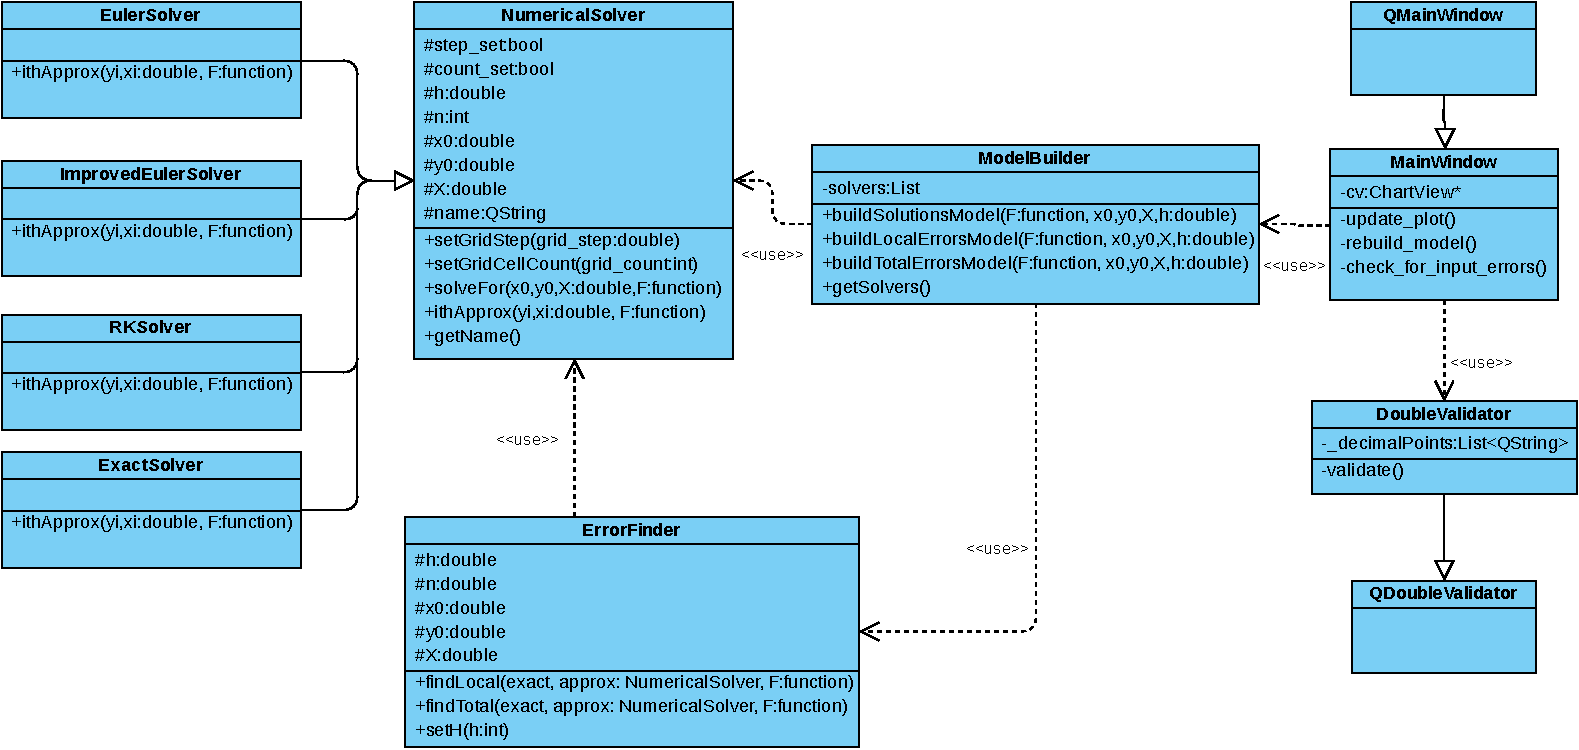
\includegraphics[width=\linewidth]{fin.pdf}

NumericalSolver class is an abstract class designed to represent  
general procedure of building numerical solution that is same for all
numerical methods for this assignment (that is Euler's method, Improved 
Euler's method and Runge-Kutta method). Classes EulerSolver, ImprovedEulerSolver
RKSolver are descendants of NumericalSolver and each of them implements
function ithApprox() in such manner that respective numerical method implies.
For example, here is the source code of function ithApprox() for EulerSolver class:
\begin{lstlisting}
double EulerSolver::ithApprox(double xi,double yi,
     double (*F)(double, double))
{
    return yi+h*(F(xi,yi));
}
\end{lstlisting}
ExactSolver is decsendant of NumericalSolver, too, however its role is return
exact solution for given IVP.

ErrorFinder class is responsible for building local and total errors
functions. The class uses two NumericalSolver's instances to build each
function: first is reference approximation (in all cases in this report exact
solution is used as a reference), and the second one is approximation itself.

ModelBuilder class is responsible for buildind models which are the part of
Model-View-Controller programming approach. Model built by ModelBuilder are used 
by MainWindow class to build plots and tables for needed functions.

MainWindow class is responsible for all UI and user interactions. Also to satisfy
regional standarts of inputting doubles (, instead of .) there was created class 
DoubleValidator that validates all double-input fields.
\subsection{Implementation of numerical methods}
The three numerical methods required in the assignment statement were
implemented. Possibility of plotting and changing initial conditions were provided 
for each method, too. Screenshots of program's work with different grid steps
amount is presented below:
\newpage
\begin{center}
\large Solutions for $N=9$
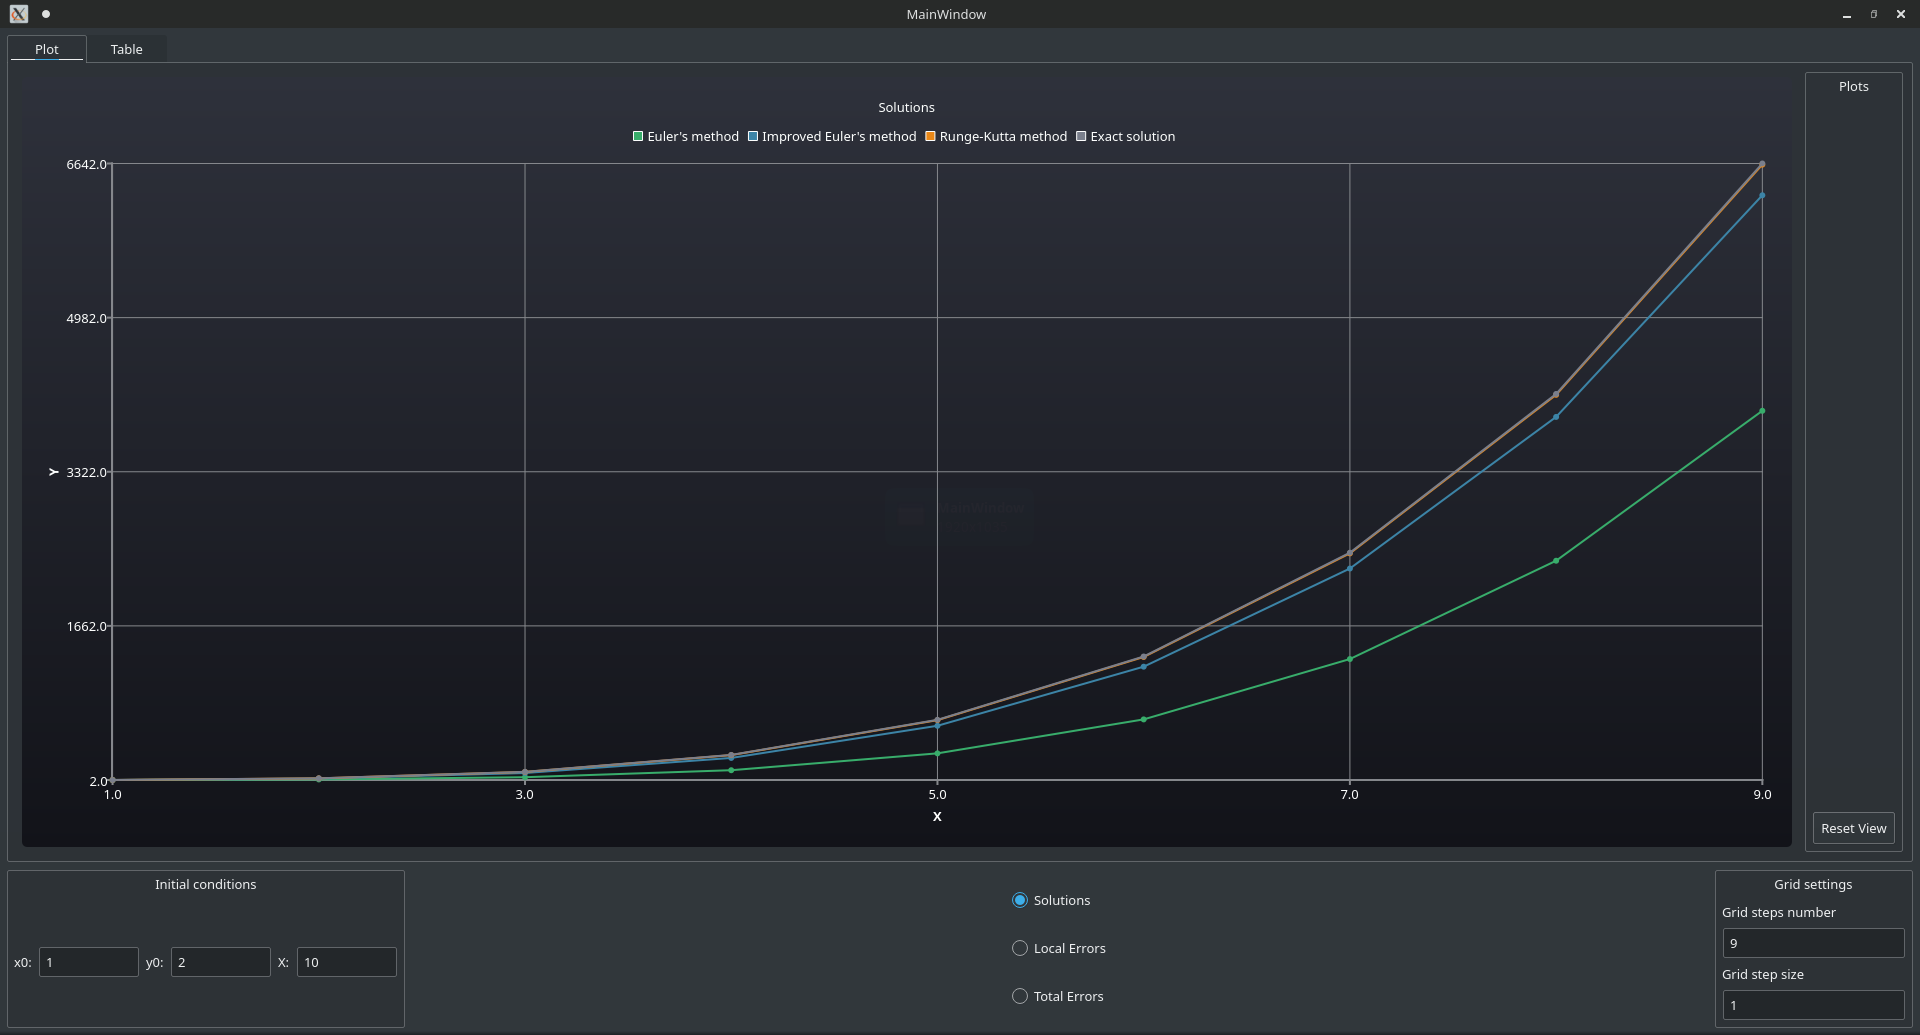
\includegraphics[width=\linewidth]{shot1.png}
\large Solutions for $N=20$
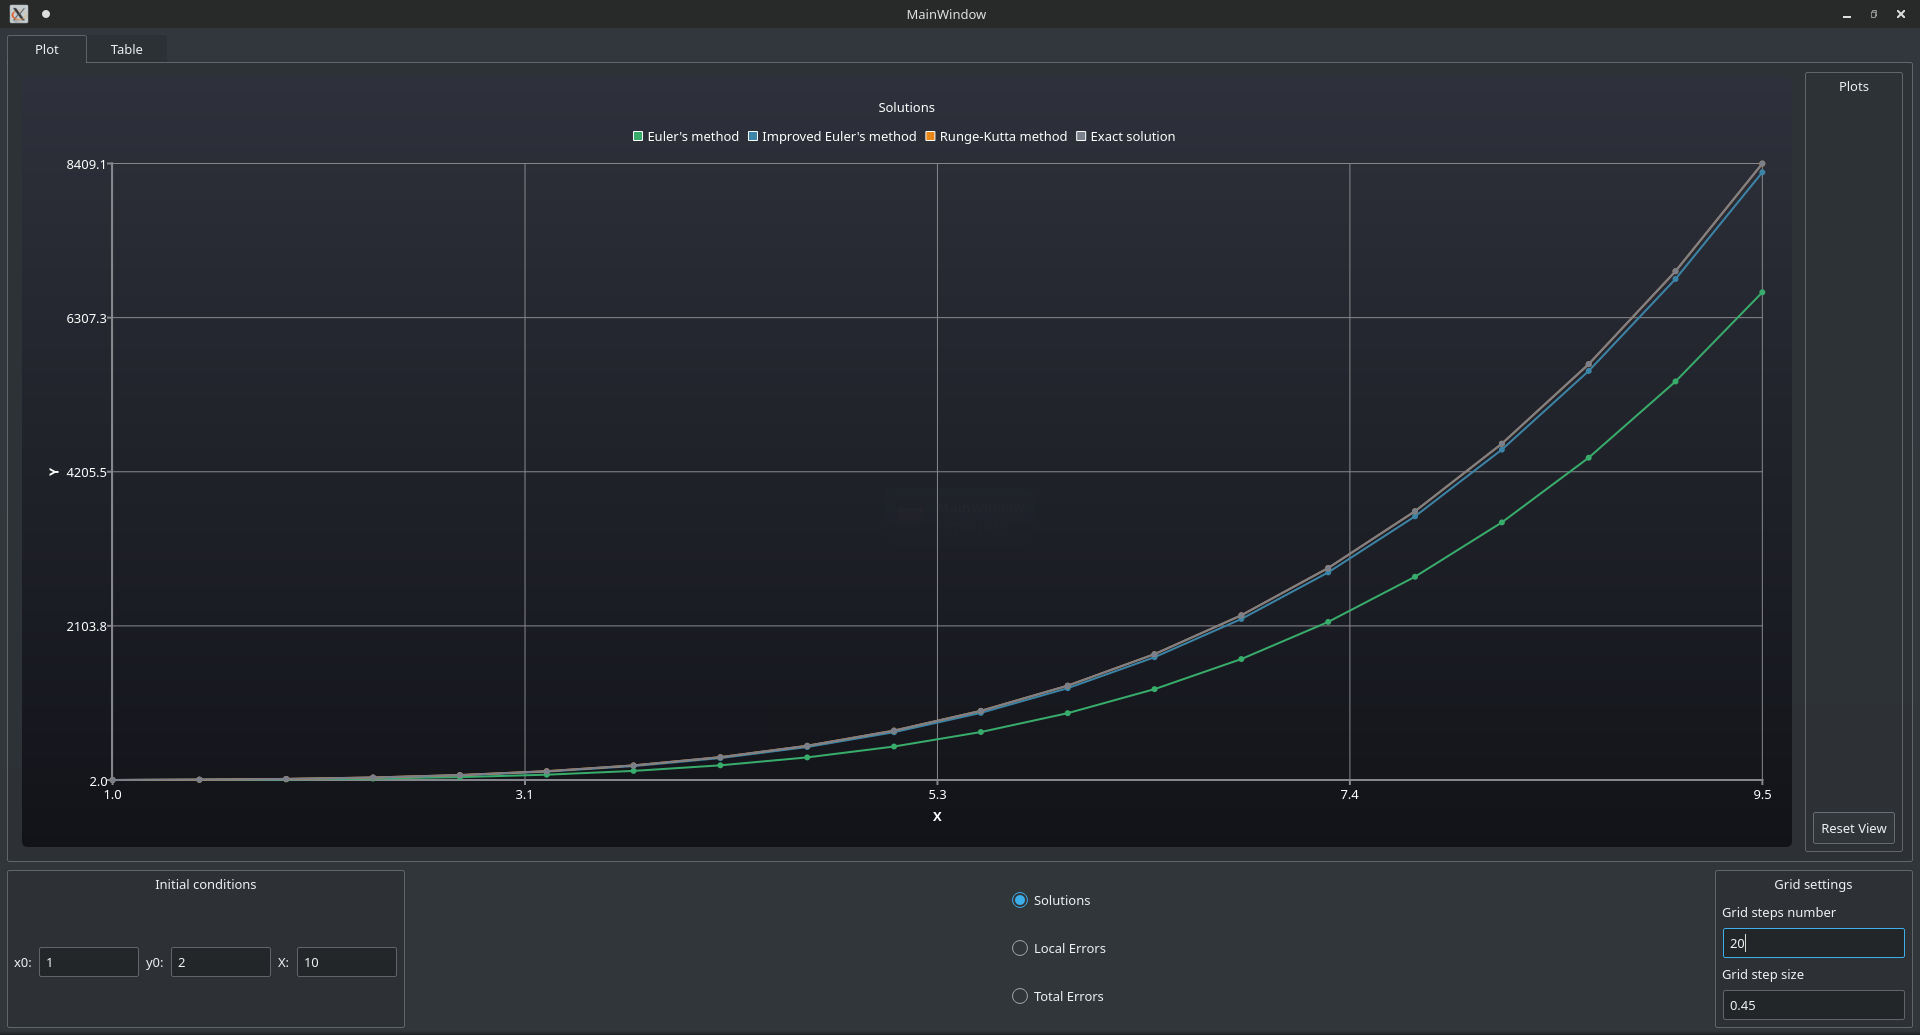
\includegraphics[width=\linewidth]{shot3.png}
\newpage
\large Solutions for $N=100$
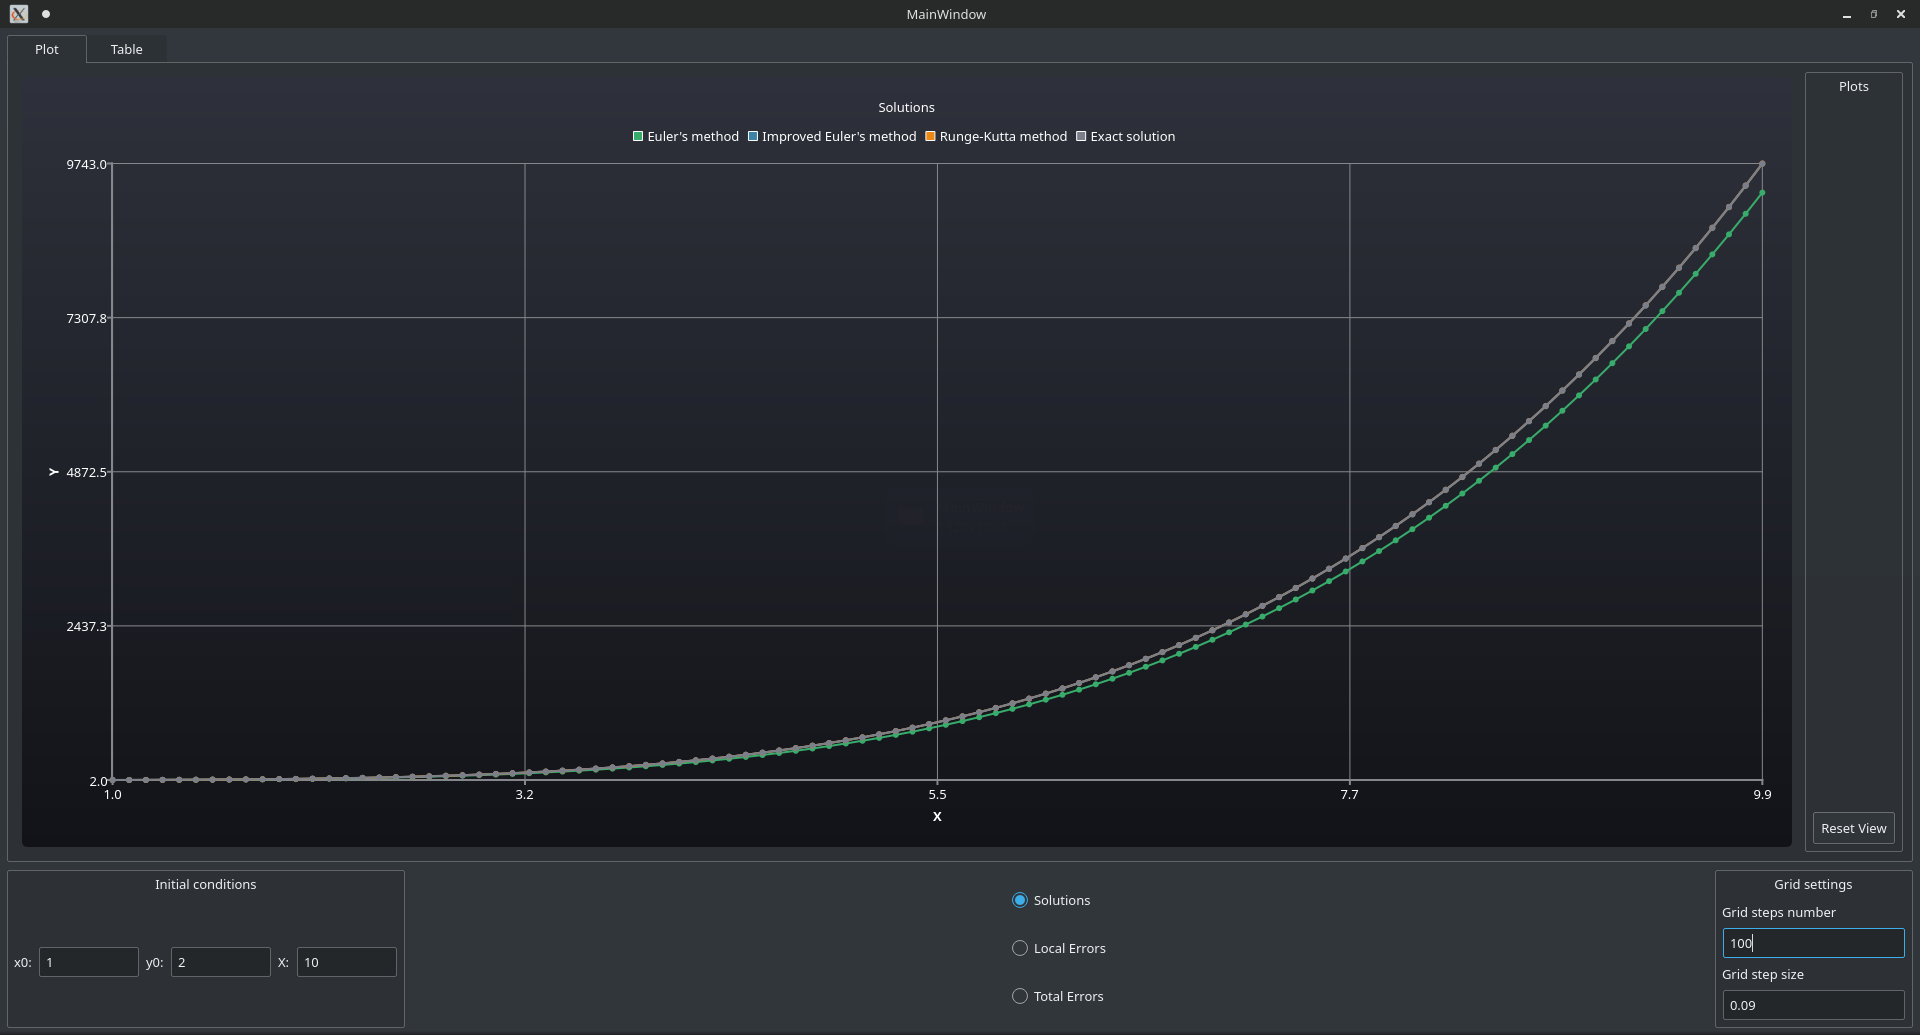
\includegraphics[width=\linewidth]{shot2.png}
\end{center}
At all screenshots plot of solution by Runge-Kutta method is almost non-visible. 
The reason behind that is that the method gives very correct approximation for this IVP and 
plot of solution is situated close to exact solution.
As can be seen from the plots, the approximation errors grows when $x$ grows.
The reason is that approximation errors has order of derivative in power $n$,
where $n$ is individual for each method, that constantly grows on interval
$x\in(-\infty;+\infty)$ for the given IVP.
\subsection{Approximation Errors}
The total approximation errors of different methods are presented at table below:\\
\begin{tabular}{|l|l|l|l|}
    \hline
                            & N=9   & N=20   & N=100   \\ \hline
    Euler's method          & 418.0 & 104.175  & 4.723     \\ \hline
    Improved Euler's method & 29.44 & 3.2092  & 0.2851   \\ \hline
    Runge-Kutta method      & 0.3472 & 0.12138 & $6.3e-6$ \\ \hline
\end{tabular}\\
As one can see from the table, error in Runge-Kutta method is the lowest;
and Euler's method has the greatest approximation error.\\
The next screenshot illustrates how total approximation error is changed with change
of number of grid cells:\\
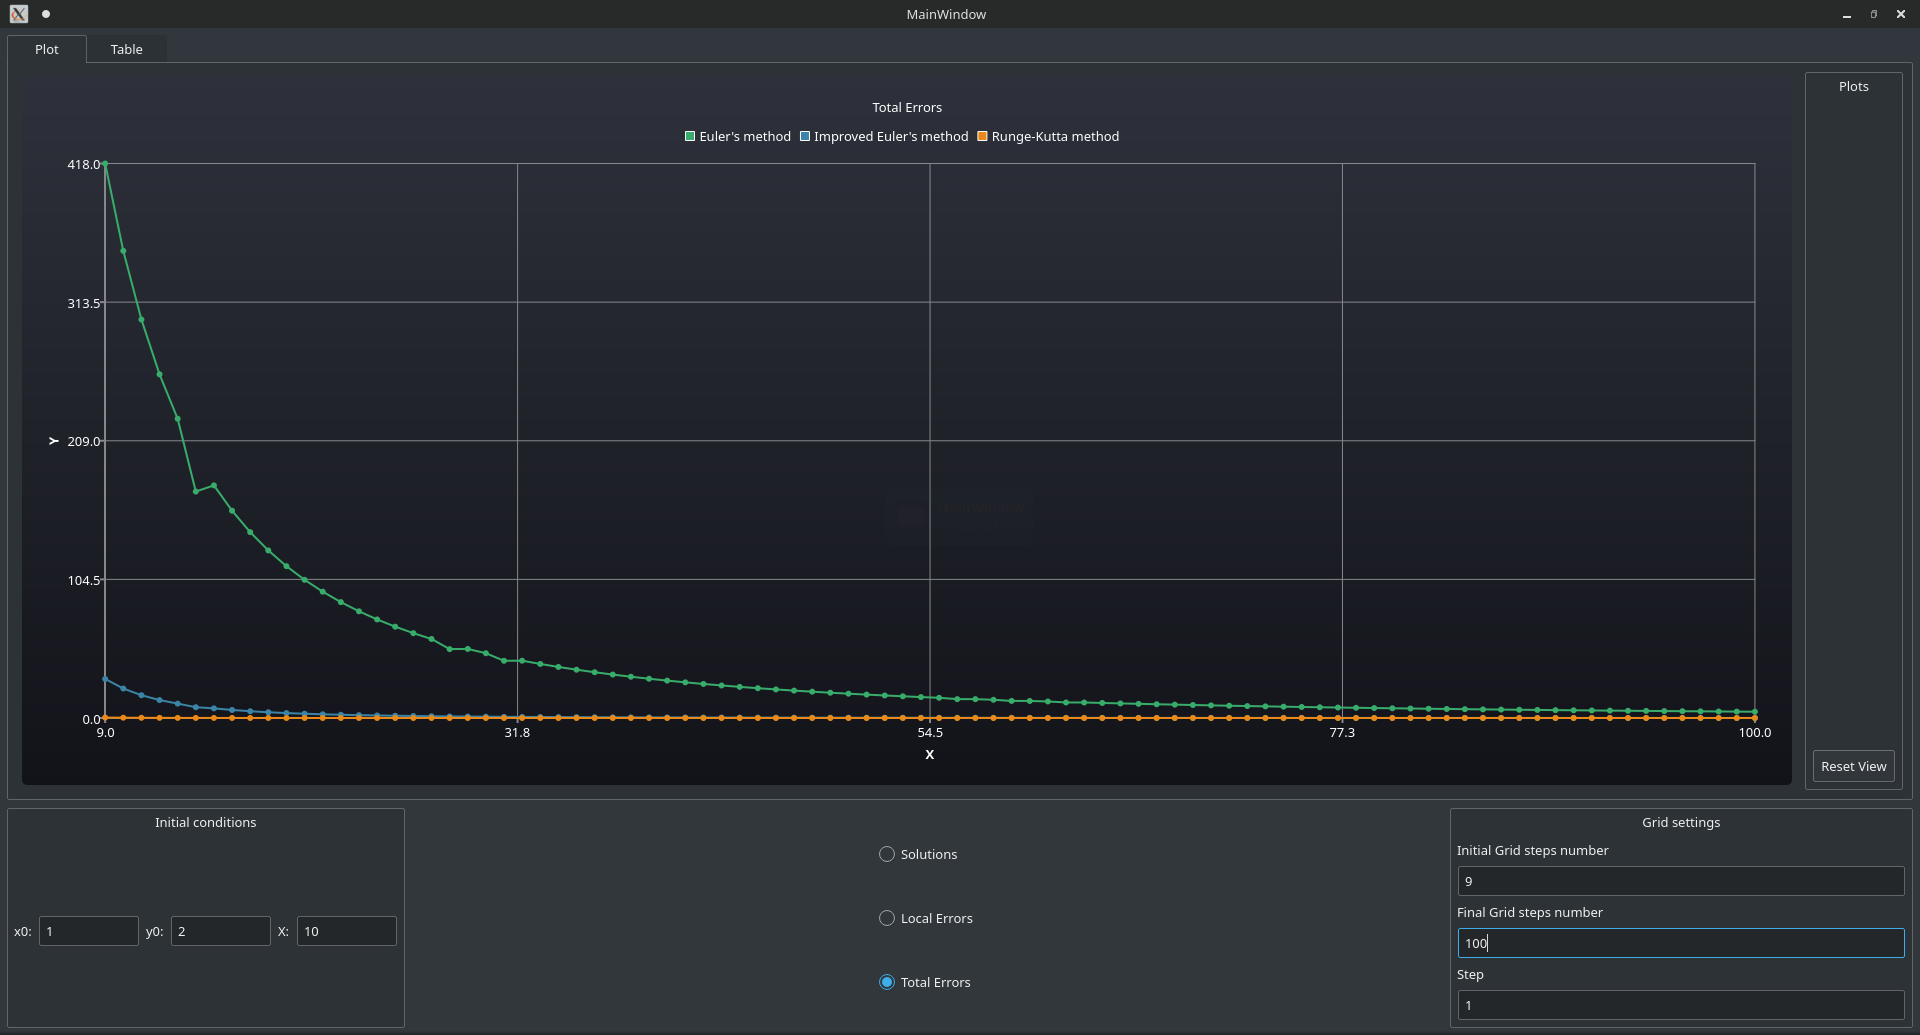
\includegraphics[width=\linewidth]{shot4.png}
As can be seen, the approximation errors are lowered.
\section{References}
\begin{enumerate}
    \item Elementary Differential Equations by William F. Trench.
    Brooks/Cole Thomson Learning, 2001.  
    \item https://doc.qt.io
    \item Moodle :)
\end{enumerate}
\end{document}